\documentclass[11pt]{ainotes}

\title{Machine Learning and Data Mining}
\date{2023 -- 2024}

\DeclareAcronym{oltp}{short=OLTP, long=Online Transaction Processing}
\DeclareAcronym{erp}{short=ERP, long=Enterprise Resource Planning}
\DeclareAcronym{mis}{short=MIS, long=Management Information System}
\DeclareAcronym{dss}{short=DSS, long=Decision Support System}
\DeclareAcronym{eis}{short=EIS, long=Executive Information System}
\DeclareAcronym{olap}{short=OLAP, long=Online Analysical Processing}
\DeclareAcronym{bi}{short=BI, long=Business Intelligence}
\DeclareAcronym{dwh}{short=DWH, long=Data Warehouse}
\DeclareAcronym{dm}{short=DM, long=Data Mart}
\DeclareAcronym{etl}{short=ETL, long=Extraction{,} Transformation{,} Loading}
\DeclareAcronym{dfm}{short=DFM, long=Dimensional Fact Model}
\DeclareAcronym{cdc}{short=CDC, long=Change Data Capture}
\DeclareAcronym{crisp}{short=CRISP-DM, long=Cross Industry Standard Process for Data Mining}


\begin{document}

    \makenotesfront
    \printacronyms
    \newpage

    \lohead{\color{gray} Not required for the exam}
\lehead{\color{gray} Not required for the exam}
\chapter{Introduction}


\section{AI systems classification}

\subsection{Intelligence classification}
Intelligence is defined as the ability to perceive or infer information and to retain the knowledge for future use.

\begin{description}
    \item[Weak AI] \marginnote{Weak AI}
        aims to build a system that acts as an intelligent system. 
    
        \item[Strong AI] \marginnote{Strong AI}
        aims to build a system that is actually intelligent. 
\end{description}


\subsection{Capability classification}
\begin{description}
    \item[General AI] \marginnote{General AI}
        systems able to solve any generalized task. 
    
        \item[Narrow AI] \marginnote{Narrow AI}
        systems able to solve a particular task. 
\end{description}


\subsection{AI approaches}
\begin{description}
    \item[Symbolic AI (top-down)] \marginnote{Symbolic AI}
        Symbolic representation of knowledge, understandable by humans.

    \item[Connectionist approach (bottom-up)] \marginnote{Connectionist approach}
        Neural networks. Knowledge is encoded and not understandable by humans.
\end{description}



\section{Symbolic AI}
\begin{description}
    \item[Deductive reasoning] \marginnote{Deductive reasoning}
        Conclude something given some premises (general to specific). 
        It is unable to produce new knowledge.
        \begin{example}
            "All men are mortal" and "Socrates is a man" $\rightarrow$ "Socrates is mortal"
        \end{example}
    
    \item[Inductive reasoning] \marginnote{Inductive reasoning}
        A conclusion is derived from an observation (specific to general).
        Produces new knowledge, but correctness is not guaranteed.
        \begin{example}
            "Several birds fly" $\rightarrow$ "All birds fly"
        \end{example}

    \item[Abduction reasoning] \marginnote{Abduction reasoning}
        An explanation of the conclusion is found from known premises.
        Differently from inductive reasoning, it does not search for a general rule.
        Produces new knowledge, but correctness is not guaranteed.
        \begin{example}
            "Socrates is dead" (conclusion) and "All men are mortal" (knowledge) $\rightarrow$ "Socrates is a man"
        \end{example}
    
    \item[Reasoning by analogy] \marginnote{Reasoning by analogy}
        Principle of similarity (e.g. k-nearest-neighbor algorithm).
        \begin{example}
            "Socrates loves philosophy" and Socrates resembles John $\rightarrow$ "John loves philosophy"
        \end{example}

    \item[Constraint reasoning and optimization] \marginnote{Constraint reasoning}
        Constraints, probability, statistics.
\end{description}


\section{Machine learning}

\subsection{Training approach}
\begin{description}
    \item[Supervised learning] \marginnote{Supervised learning}
        Trained on labeled data (ground truth is known).\\
        Suitable for classification and regression tasks.

    \item[Unsupervised learning] \marginnote{Unsupervised learning}
        Trained on unlabeled data (the system makes its own discoveries).\\
        Suitable for clustering and data mining.

    \item[Semi-supervised learning] \marginnote{Semi-supervised learning}
        The system is first trained to synthesize data in an unsupervised manner,
        followed by a supervised phase.

    \item[Reinforcement learning] \marginnote{Reinforcement learning}
        An agent learns by simulating actions in an environment with rewards and punishments depending on its choices.
\end{description}


\subsection{Tasks}
\begin{description}
    \item[Classification] \marginnote{Classification}
        Supervised task that, given the input variables $X$ and the output (discrete) categories $Y$,
        aims to approximate a mapping function $f: X \rightarrow Y$.

    \item[Regression] \marginnote{Regression}
        Supervised task that, given the input variables $X$ and the output (continuous) variables $Y$,
        aims to approximate a mapping function $f: X \rightarrow Y$.

    \item[Clustering] \marginnote{Clustering}
        Unsupervised task that aims to organize objects into groups.
\end{description}


\subsection{Neural networks}
\marginnote{Perceptron}
A neuron (\textbf{perceptron}) computes a weighted sum of its inputs and 
passes the result to an activation function to produce the output.
\begin{figure}[h]
    \centering
    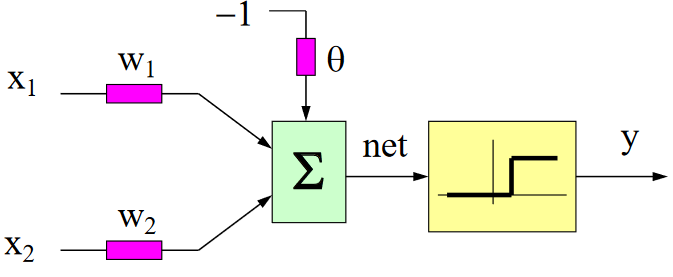
\includegraphics[width=0.40\textwidth]{img/neuron.png}
    \caption{Representation of an artificial neuron}
\end{figure}

\marginnote{Feed-forward neural network}
A \textbf{feed-forward neural network} is composed of multiple layers of neurons, each connected to the next one.
The first layer is the input layer, while the last is the output layer.
Intermediate layers are hidden layers.

The expressivity of a neural network increases when more neurons are used:
\begin{descriptionlist}
    \item[Single perceptron] 
        Able to compute a linear separation.
        \begin{figure}[h]
            \centering
            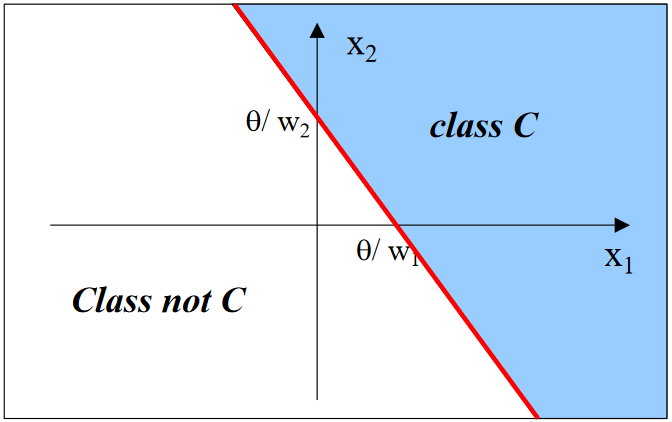
\includegraphics[width=0.25\textwidth]{img/1perceptron.png}
            \caption{Separation performed by one perceptron}
        \end{figure}
    \item[Three-layer network] 
        Able to separate a convex region ($n_\text{edges} \leq n_\text{hidden neurons}$)
        \begin{figure}[h]
            \centering
            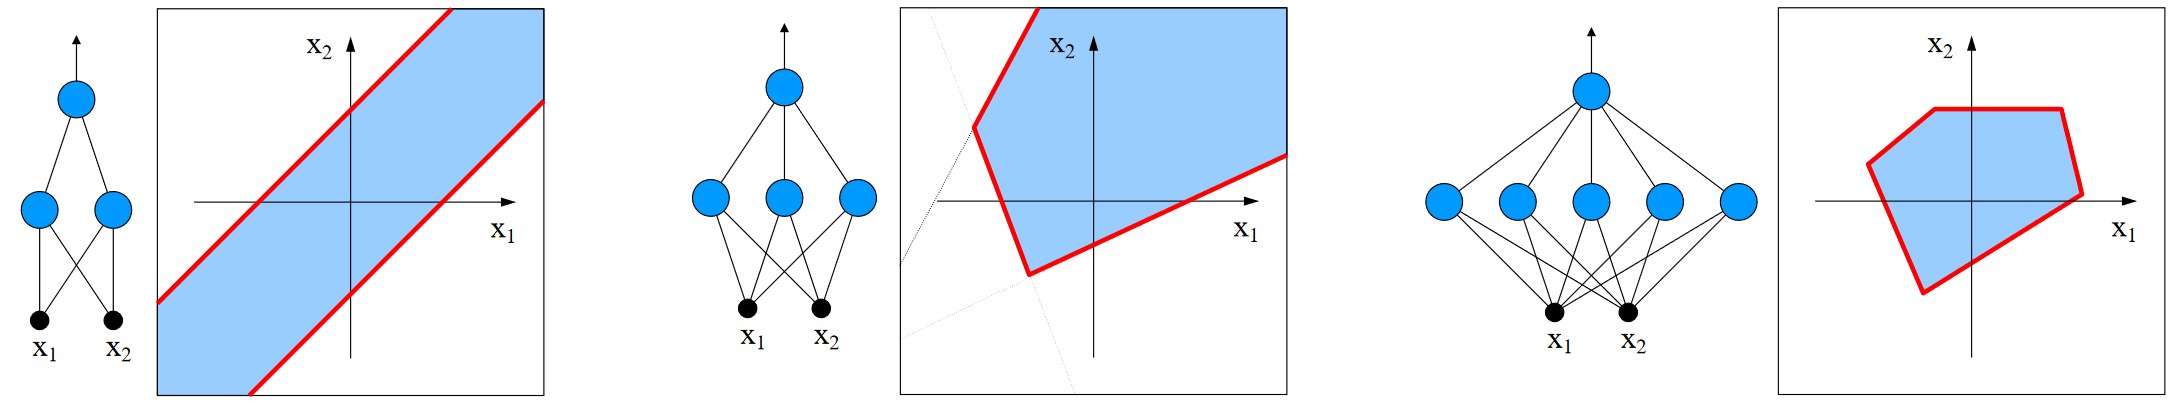
\includegraphics[width=0.90\textwidth]{img/3layer.png}
            \caption{Separation performed by a three-layer network}
        \end{figure}
    \item[Four-layer network] 
        Able to separate regions of arbitrary shape.
        \begin{figure}[h]
            \centering
            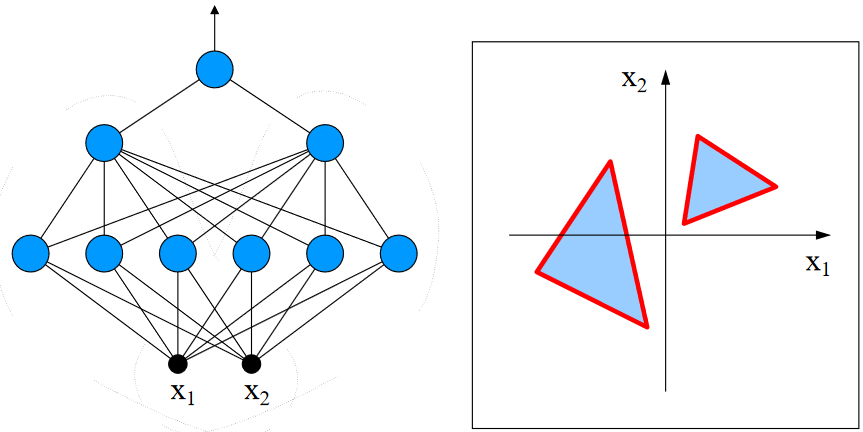
\includegraphics[width=0.40\textwidth]{img/4layer.png}
            \caption{Separation performed by a four-layer network}
        \end{figure}
\end{descriptionlist}

\begin{theorem}[Universal approximation theorem] \marginnote{Universal approximation theorem}
    A feed-forward network with one hidden layer and a finite number of neurons is
    able to approximate any continuous function with desired accuracy.
\end{theorem}

\begin{description}
    \item[Deep learning] \marginnote{Deep learning}
        Neural network with a large number of layers and neurons.
        The learning process is hierarchical: the network exploits simple features in the first layers and
        synthesizes more complex concepts while advancing through the layers.
\end{description}



\section{Automated planning}
Given an initial state, a set of actions and a goal, 
\textbf{automated planning} aims to find a partially or totally ordered sequence of actions to achieve a goal. \marginnote{Automated planning}

An \textbf{automated planner} is an agent that operates in a given domain described by:
\begin{itemize}
    \item Representation of the initial state
    \item Representation of a goal
    \item Formal description of the possible actions (preconditions and effects)
\end{itemize}



\section{Swarm intelligence}
\marginnote{Swarm intelligence}
Decentralized and self-organized systems that result in emergent behaviors. 



\section{Decision support systems}

\begin{description}
    \item[Knowledge based system] \marginnote{Knowledge based system}
        Use knowledge (and data) to support human decisions.
        Bottlenecked by knowledge acquisition.
\end{description}

Different levels of decision support exist:
\begin{descriptionlist}
    \item[Descriptive analytics] \marginnote{Descriptive analytics}
        Data are used to describe the system (e.g. dashboards, reports, \dots).
        Human intervention is required.
            
    \item[Diagnostic analytics] \marginnote{Diagnostic analytics}
        Data are used to understand causes (e.g. fault diagnosis)
        Decisions are made by humans.

    \item[Predictive analytics] \marginnote{Predictive analytics}
        Data are used to predict future evolutions of the system.
        Uses machine learning models or simulators (digital twins)

    \item[Prescriptive analytics] \marginnote{Prescriptive analytics}
        Make decisions by finding the preferred scenario.
        Uses optimization systems, combinatorial solvers or logical solvers.
\end{descriptionlist}


\newpage
\lohead{}
\lehead{}

    \chapter{Data warehouse}


\begin{description}
    \item[\Acl{bi}] \marginnote{\Acl{bi}}
        Transform raw data into information.
        Deliver the right information to the right people at the right time through the right channel.

    \item[\Ac{dwh}] \marginnote{\Acl{dwh}}
        Optimized repository that stores information for decision-making processes.
        \Acp{dwh} are a specific type of \ac{dss}.

        Features:
        \begin{itemize}
            \item Subject-oriented: focused on enterprise-specific concepts.
            \item Integrates data from different sources and provides a unified view.
            \item Non-volatile storage with change tracking. 
        \end{itemize}

    \item[\Ac{dm}] \marginnote{\Acl{dm}}
        Subset of the primary \ac{dwh} with information relevant to a specific business area.
\end{description}



\section{\Acl{olap} (\Acs{olap})}

\begin{description}
    \item[\ac{olap} analyses] \marginnote{\Acl{olap} (\Acs{olap})}
        Able to interactively navigate the information in a data warehouse.
        Allows to visualize different levels of aggregation.

    \item[\ac{olap} session] 
        Navigation path created by the operations that a user applied.
\end{description}

\begin{figure}[ht]
    \centering
    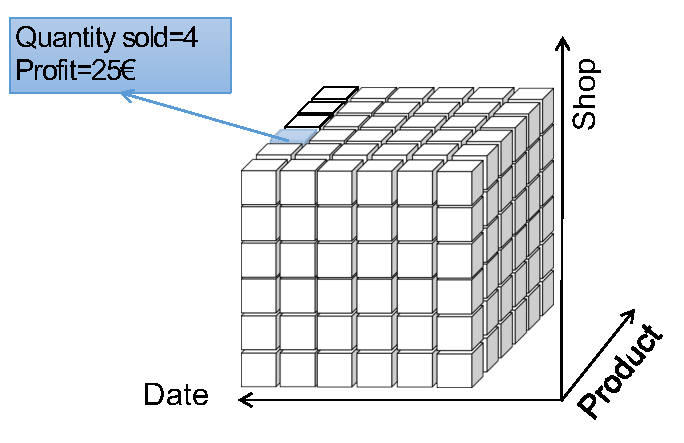
\includegraphics[width=0.35\textwidth]{img/_olap_cube.pdf}
    \caption{\ac{olap} data cube}
\end{figure}


\subsection{Operators}

\begin{description}
    \item[Roll-up] \marginnote{Roll-up}
        \begin{minipage}{0.7\textwidth}
            Increases the level of aggregation (i.e. \texttt{GROUP BY} in SQL).
            Some details are collapsed together.
        \end{minipage}
        \hfill
        \begin{minipage}{0.15\textwidth}
            \centering
            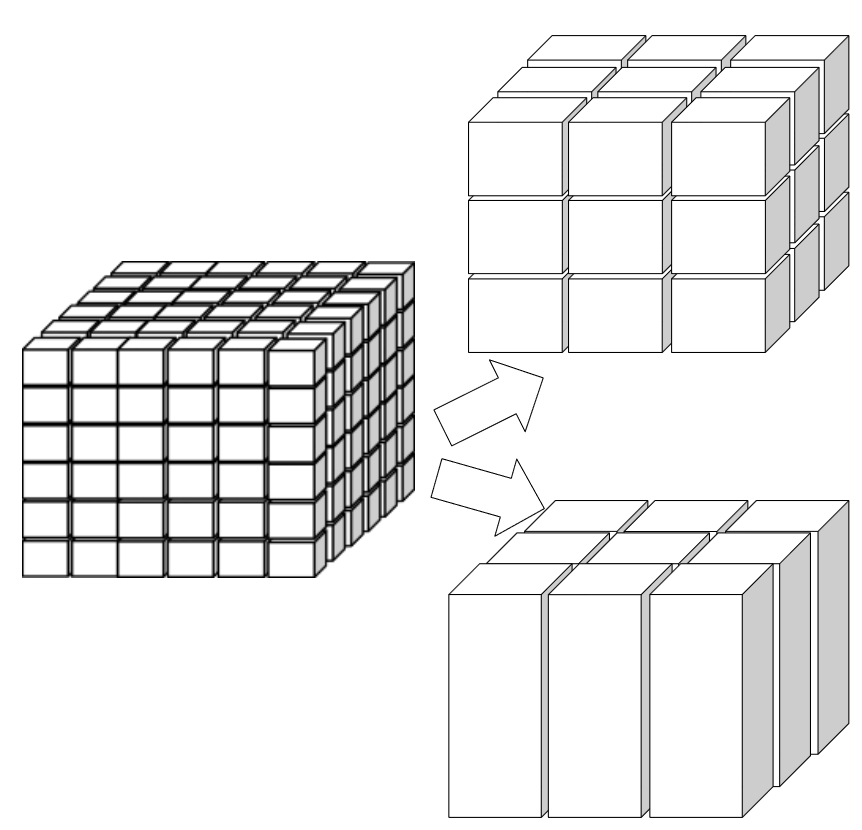
\includegraphics[width=\linewidth]{img/olap_rollup.png}
        \end{minipage}

    \item[Drill-down] \marginnote{Drill-down}
        \begin{minipage}{0.7\textwidth}
            Reduces the level of aggregation.
            Some details are reintroduced.
        \end{minipage}
        \hfill
        \begin{minipage}{0.15\textwidth}
            \centering
            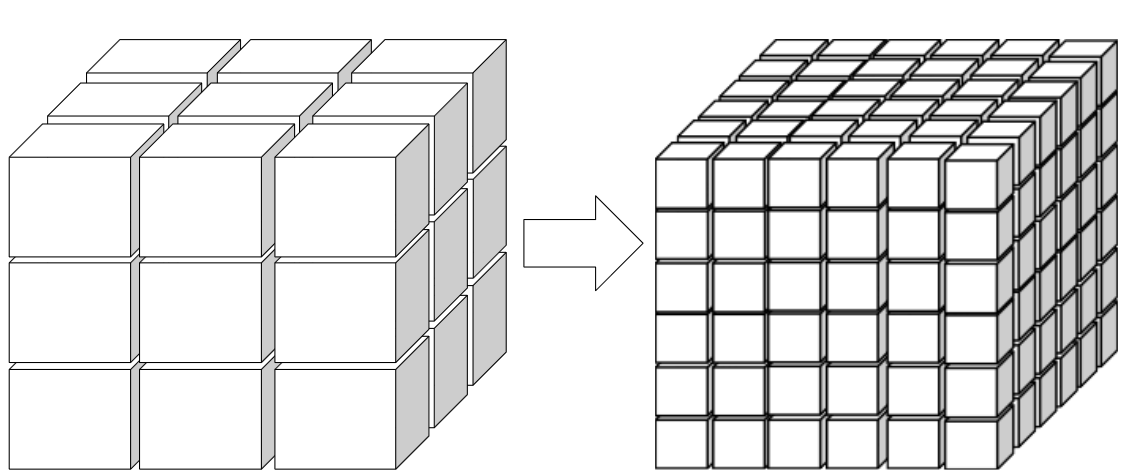
\includegraphics[width=\linewidth]{img/olap_drilldown.png}
        \end{minipage}
    
    \item[Slide-and-dice] \marginnote{Slide-and-dice}
        \begin{minipage}{0.65\textwidth}
            The slice operator reduces the number of dimensions (i.e. drops columns).

            The dice operator reduces the number of data being analyzed (i.e. \texttt{LIMIT} in SQL).
        \end{minipage}
        \hfill
        \begin{minipage}{0.15\textwidth}
            \centering
            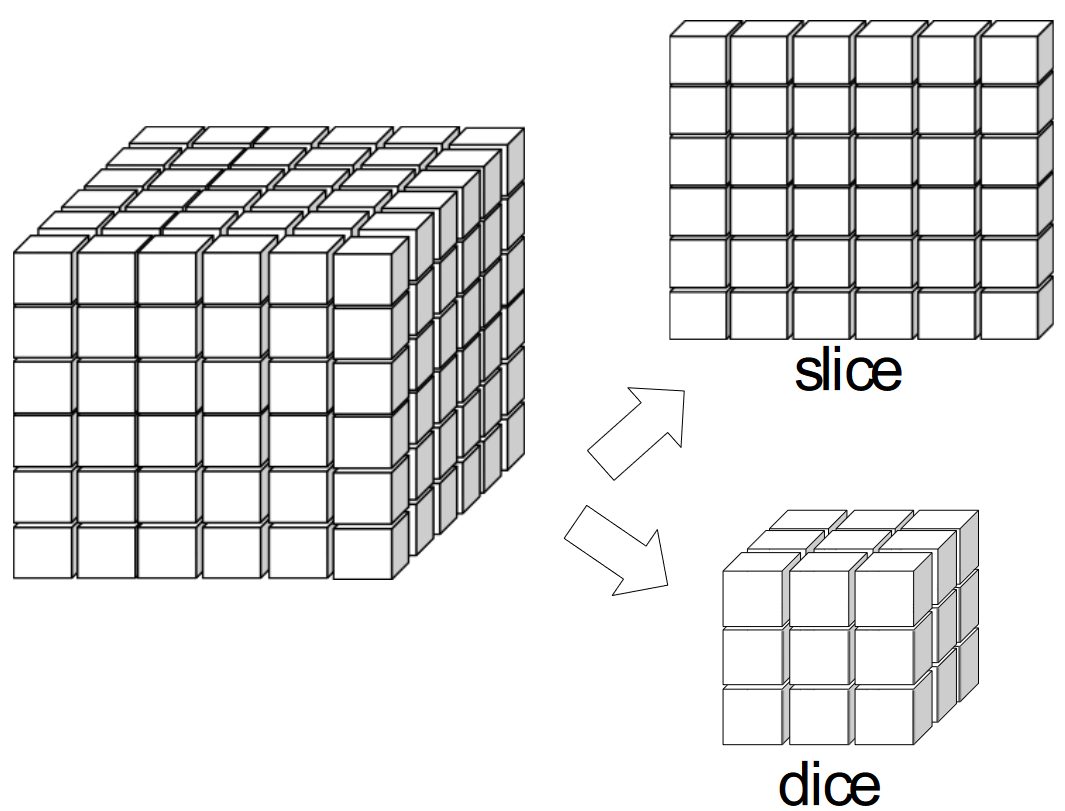
\includegraphics[width=\linewidth]{img/olap_slicedice.png}
        \end{minipage}    

    \item[Pivot] \marginnote{Pivot}
        \begin{minipage}{0.7\textwidth}
            Changes the layout of the data, to analyze it from a different viewpoint.
        \end{minipage}
        \hfill
        \begin{minipage}{0.15\textwidth}
            \centering
            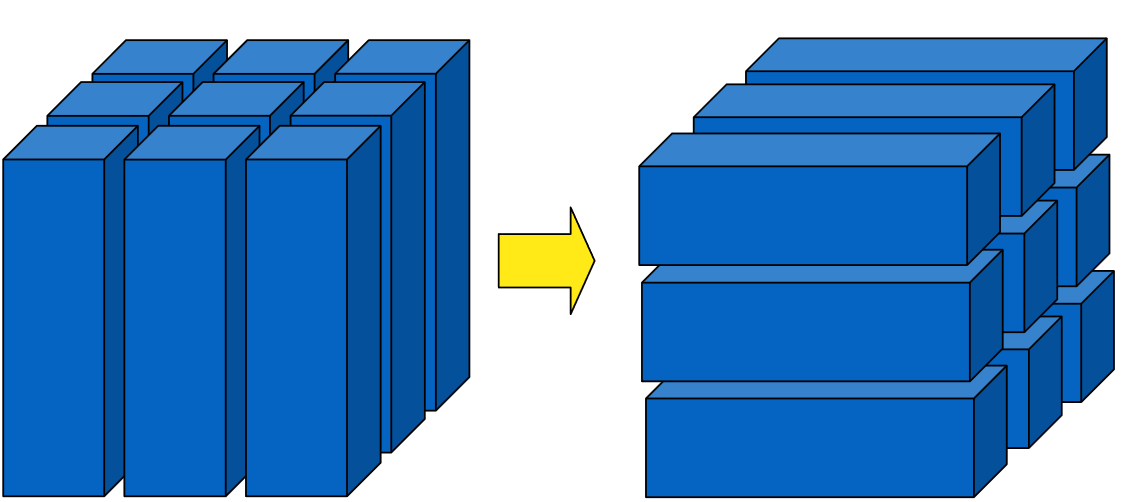
\includegraphics[width=\linewidth]{img/olap_pivot.png}
        \end{minipage}

    \item[Drill-across] \marginnote{Drill-across}
        \begin{minipage}{0.7\textwidth}
            Links concepts from different data sources (i.e. \texttt{JOIN} in SQL).
        \end{minipage}
        \hfill
        \begin{minipage}{0.15\textwidth}
            \centering
            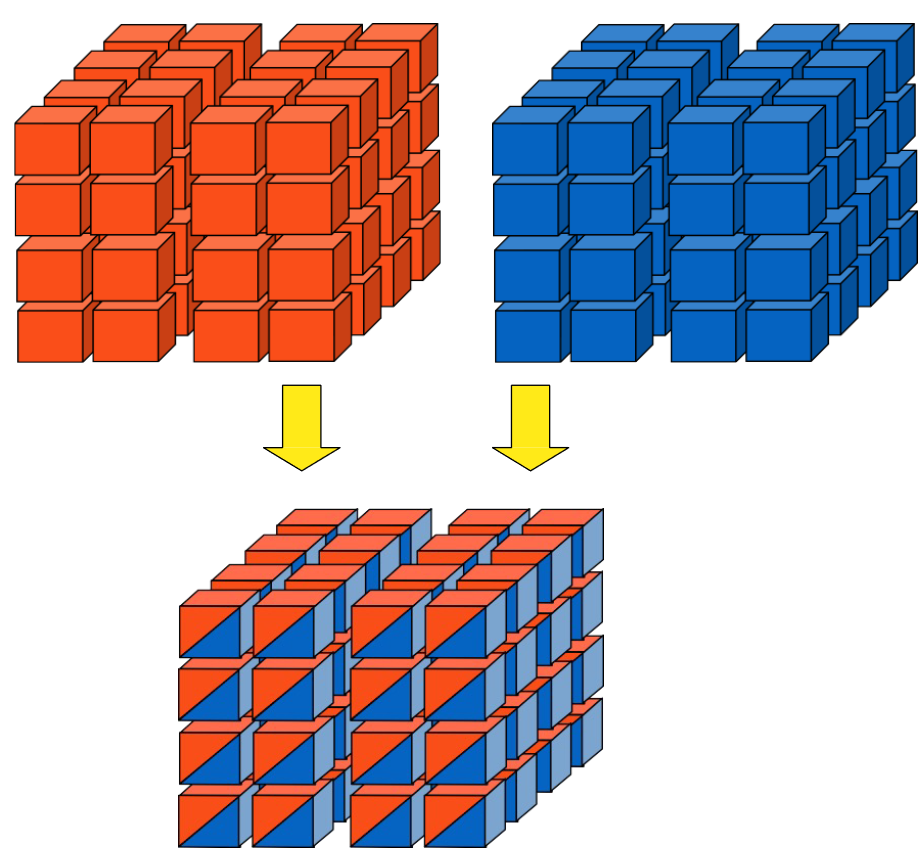
\includegraphics[width=\linewidth]{img/olap_drillacross.png}
        \end{minipage}    
    
    \item[Drill-through] \marginnote{Drill-through}
        Switches from multidimensional aggregated data to operational data (e.g. a spreadsheet).
        \begin{center}
            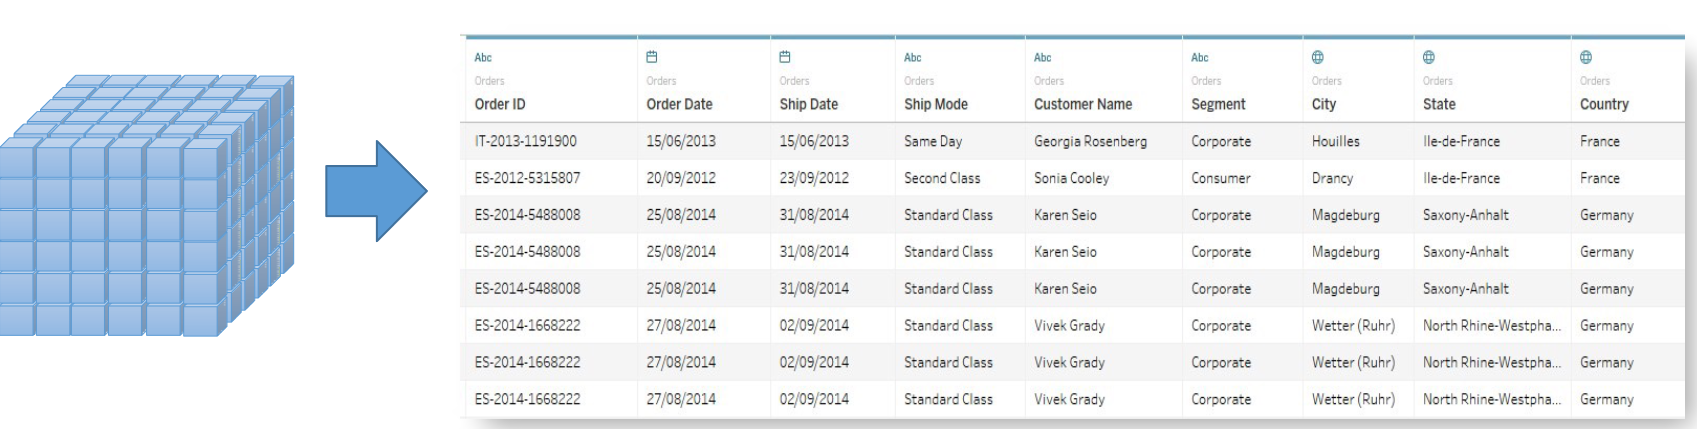
\includegraphics[width=0.5\textwidth]{img/olap_drillthrough.png}
        \end{center}    
\end{description}



\section{\Acl{etl} (\Acs{etl})}
\marginnote{\Acl{etl} (\Acs{etl})}
The \Ac{etl} process extracts, integrates and cleans operational data that will be loaded into a data warehouse.


\subsection{Extraction}

Extracted operational data can be:
\begin{descriptionlist}
    \item[Structured] \marginnote{Strucured data}
        with a predefined data model (e.g. relational DB, CSV)

    \item[Untructured] \marginnote{Unstrucured data}
        without a predefined data model (e.g. social media content)
\end{descriptionlist}

Extraction can be of two types:
\begin{descriptionlist}
    \item[Static] \marginnote{Static extraction}
        The entirety of the operational data are extracted to populate the
        data warehouse for the first time.
    
    \item[Incremental] \marginnote{Incremental extraction}
        Only changes applied since the last extraction are considered.
        Can be based on a timestamp or a trigger.
\end{descriptionlist}


\subsection{Cleaning}

Operational data may contain:
\begin{descriptionlist}
    \item[Duplicate data] 
    \item[Missing data] 
    \item[Improper use of fields] (e.g. saving the phone number in the \texttt{notes} field)
    \item[Wrong values] (e.g. 30th of February)
    \item[Inconsistencies] (e.g. use of different abbreviations)
    \item[Typos]    
\end{descriptionlist}

Methods to clean and increase the quality of the data are:
\begin{descriptionlist}
    \item[Dictionary-based techniques] \marginnote{Dictionary-based cleaning}
        Lookup tables to substitute abbreviations, synonyms or typos.
        Applicable if the domain is known and limited.
        
    \item[Approximate merging] \marginnote{Approximate merging}
        Methods to merge data that do not have a common key.
        \begin{description}
            \item[Approximate join]
                Use non-key attributes to join two tables (e.g. using the name and surname instead of a unique identifier).

            \item[Similarity approach]
                Use similarity functions (e.g. edit distance) to merge multiple instances of the same information
                (e.g. typo in customer surname).
        \end{description}
    
    \item[Ad-hoc algorithms] \marginnote{Ad-hoc algorithms}
\end{descriptionlist}


\subsection{Transformation}
Data are transformed to respect the format of the data warehouse:
\begin{descriptionlist}
    \item[Conversion] \marginnote{Conversion}
        Modifications of types and formats (e.g. date format)
    
    \item[Enrichment] \marginnote{Enrichment}
        Creating new information by using existing attributes (e.g. compute profit from receipts and expenses)

    \item[Separation and concatenation] \marginnote{Separation and concatenation}
        Denormalization of the data: introduces redundancies (i.e. breaks normal form\footnote{\url{https://en.wikipedia.org/wiki/Database_normalization}}) 
        to speed up operations.
\end{descriptionlist}


\subsection{Loading}
Adding data into a data warehouse:
\begin{descriptionlist}
    \item[Refresh] \marginnote{Refresh loading}
        The entire \ac{dwh} is rewritten.

    \item[Update] \marginnote{Update loading}
        Only the changes are added to the \ac{dwh}. Old data are not modified.
\end{descriptionlist}



\section{Data warehouse architectures}

The architecture of a data warehouse should meet the following requirements:
\begin{descriptionlist}
    \item[Separation] Separate the analytical and transactional workflows.
    \item[Scalability] Hardware and software should be easily upgradable.
    \item[Extensibility] Capability to host new applications and technologies without the need to redesign the system.
    \item[Security] Access control.
    \item[Administrability] Easily manageable.
\end{descriptionlist}

\subsection{Single-layer architecture}
\marginnote{Single-layer architecture}
\begin{minipage}{0.55\textwidth}
    \begin{itemize}
        \item Minimizes the amount of data stored (i.e. no redundances).
        \item The source layer is the only physical layer (i.e. no separation).
        \item A middleware provides the \ac{dwh} features.
    \end{itemize}
\end{minipage}
\hfill
\begin{minipage}{0.4\textwidth}
    \centering
    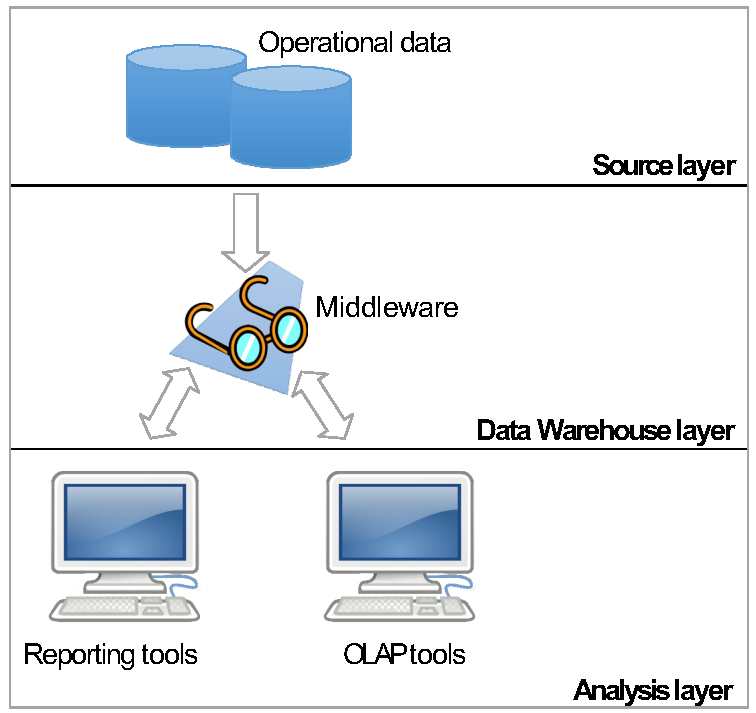
\includegraphics[width=\linewidth]{img/_1layer_dwh.pdf}
\end{minipage}


\subsection{Two-layer architecture}
\marginnote{Two-layer architecture}
\begin{minipage}{0.55\textwidth}
    \begin{itemize}
        \item Source data (source layer) are physically separated from the \ac{dwh} (data warehouse layer).
        \item A staging layer applies \ac{etl} procedures before populating the \ac{dwh}.
        \item The \ac{dwh} is a centralized repository from which data marts can be created.
            Metadata repositories store information on sources, staging and data marts schematics.
    \end{itemize}
\end{minipage}
\hfill
\begin{minipage}{0.4\textwidth}
    \centering
    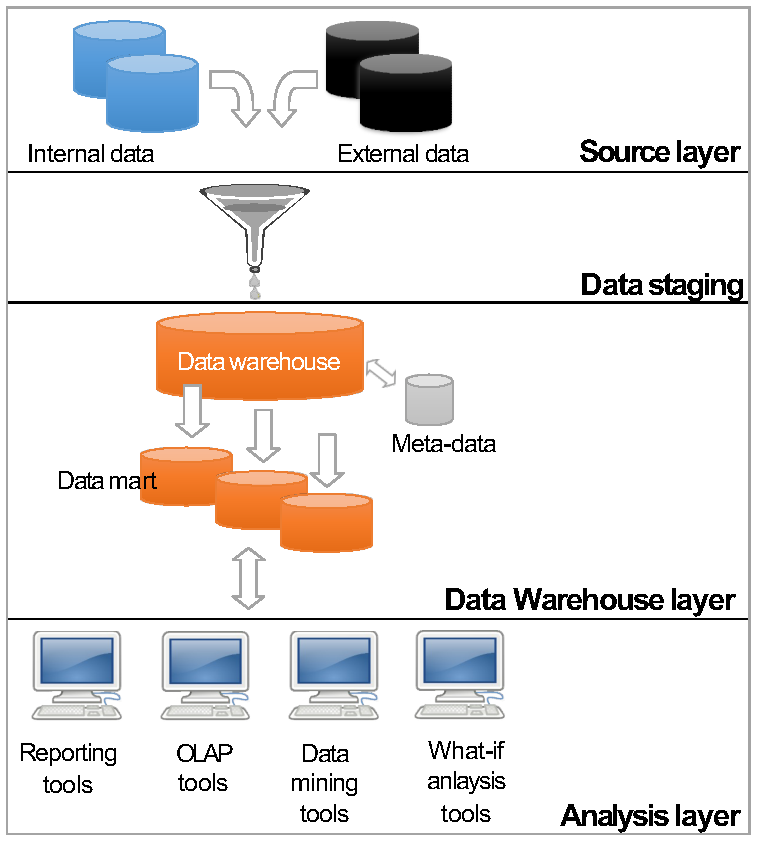
\includegraphics[width=\linewidth]{img/_2layer_dwh.pdf}
\end{minipage}


\subsection{Three-layer architecture}
\marginnote{Three-layer architecture}
\begin{minipage}{0.45\textwidth}
    \begin{itemize}
        \item A reconciled layer enhances the cleaned data coming from the staging step by 
            adding enterprise-level details (i.e. adds more redundancy before populating the \ac{dwh}).
    \end{itemize}
\end{minipage}
\hfill
\begin{minipage}{0.5\textwidth}
    \centering
    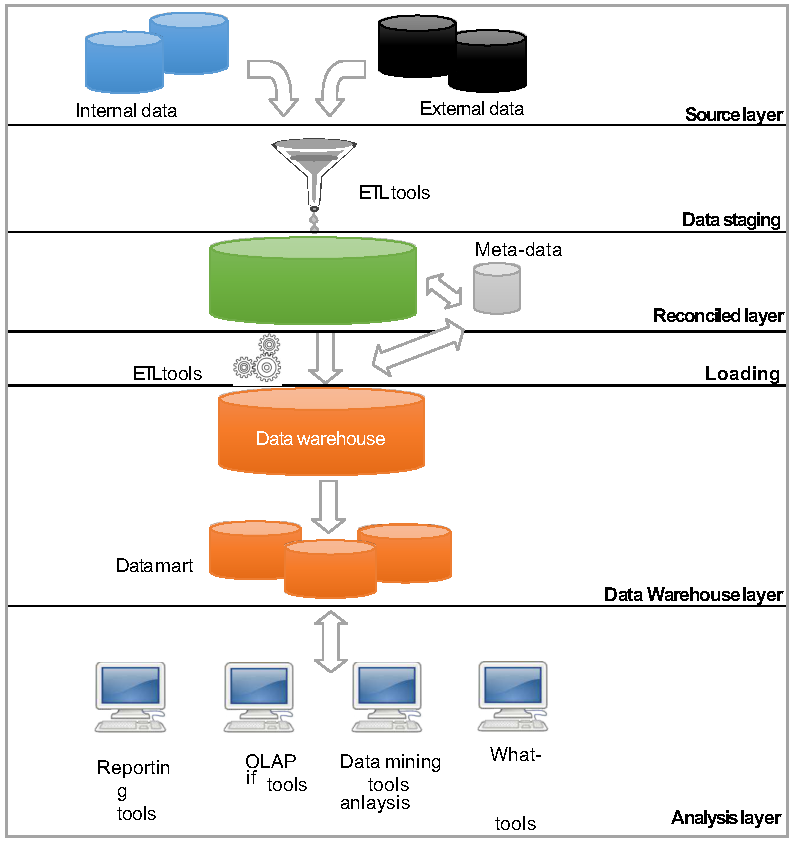
\includegraphics[width=\linewidth]{img/_3layer_dwh.pdf}
\end{minipage}



\section{Conceptual modeling}

\begin{description}
    \item[\Acl{dfm} (\acs{dfm})] \marginnote{\Acl{dfm} (\acs{dfm})}
        Conceptual model to support the design of data marts.
        The main concepts are:
        \begin{descriptionlist}
            \item[Fact] 
                Concept relevant to decision-making processes (e.g. sales).
            \item[Measure]
                Numerical property to describe a fact (e.g. profit).
            \item[Dimension] 
                Property of a fact with a finite domain (e.g. date).
            \item[Dimensional attribute] 
                Property of a dimension (e.g. month).
            \item[Hierarchy] 
                A tree where the root is a dimension and nodes are dimensional attributes (e.g. date $\rightarrow$ month).
            \item[Primary event] 
                Occurrence of a fact. It is described by a tuple with a value for each dimension and each measure.
            \item[Secondary event] 
                Aggregation of primary events. 
                Measures of primary events are aggregated if they have the same (preselected) dimensional attributes.
        \end{descriptionlist}
\end{description}

\begin{figure}[ht]
    \centering
    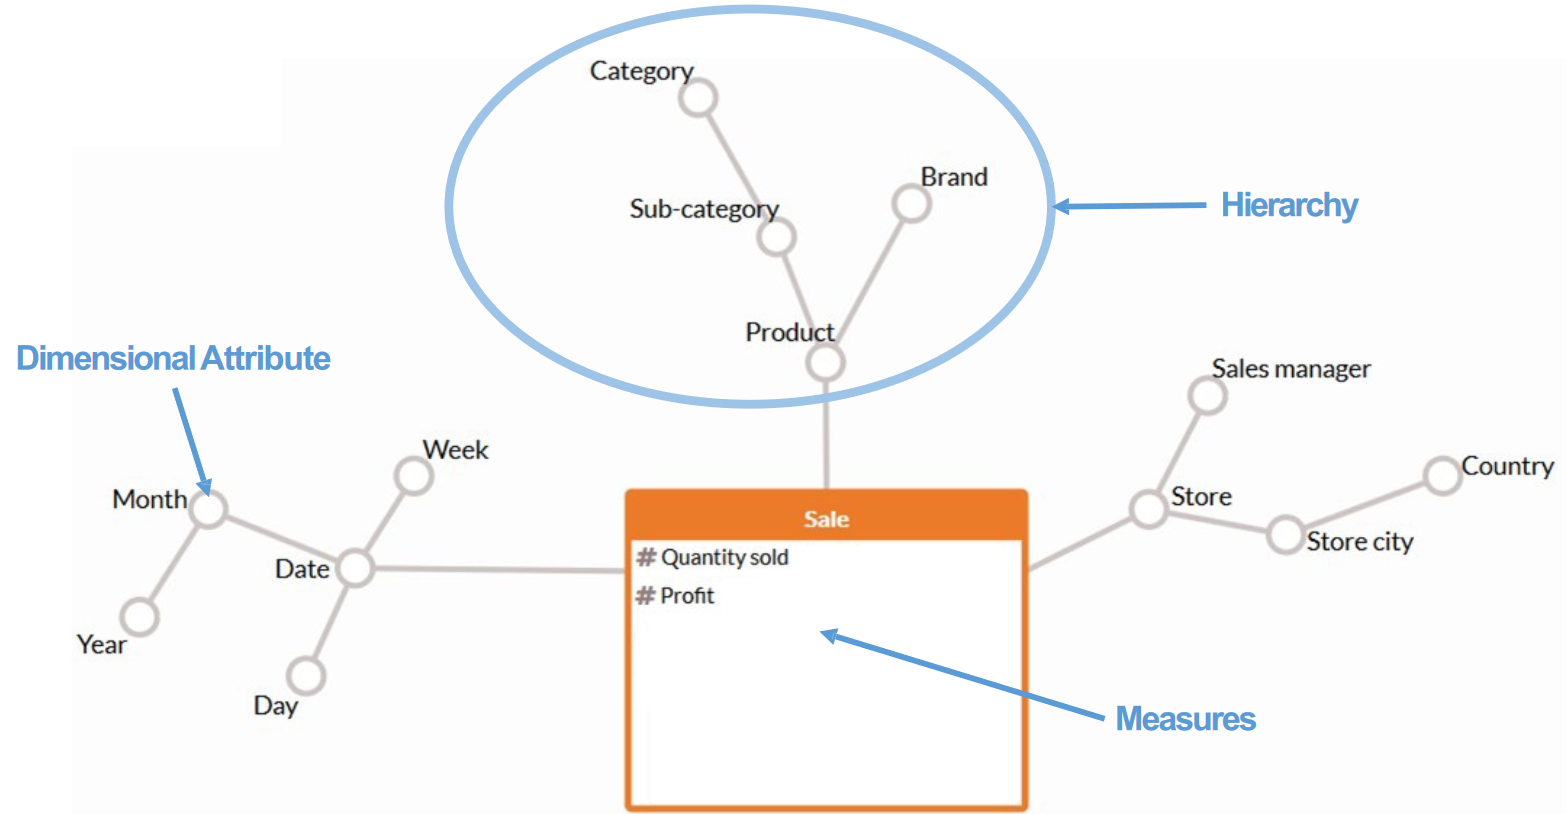
\includegraphics[width=0.8\textwidth]{img/dfm.png}
    \caption{Example of \ac{dfm}}
\end{figure}

\begin{figure}[ht]
    \centering
    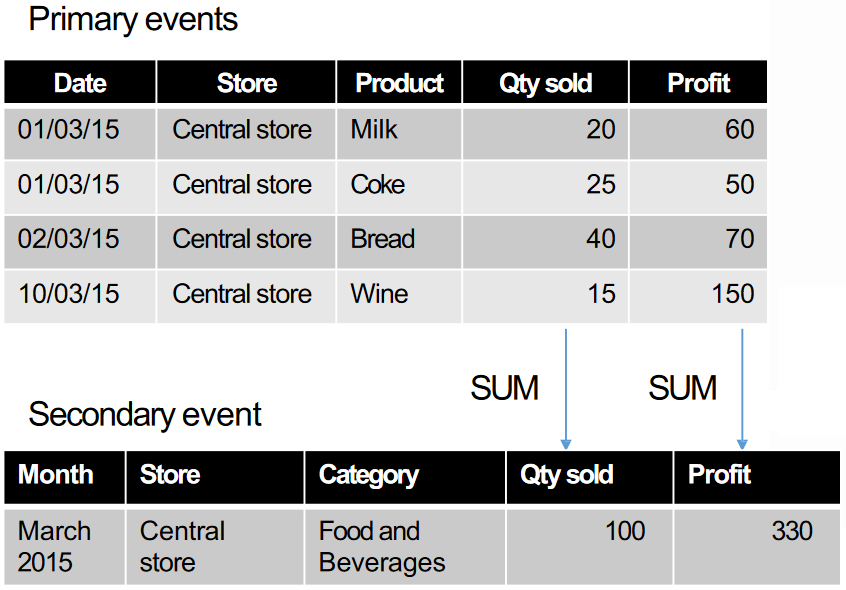
\includegraphics[width=0.5\textwidth]{img/dfm_events.png}
    \caption{Example of primary and secondary events}
\end{figure}


\subsection{Aggregation operators}

Measures can be classified as:
\begin{descriptionlist}
    \item[Flow measures] \marginnote{Flow measures}
        Evaluated cumulatively with respect to a time interval (e.g. quantity sold).
    \item[Level measures] \marginnote{Level measures}
        Evaluated at a particular time (e.g. number of products in inventory).
    \item[Unit measures] \marginnote{Unit measures}
        Evaluated at a particular time but expressed in relative terms (e.g. unit price).
\end{descriptionlist}

Aggregation operators can be classified as:
\begin{descriptionlist}
    \item[Distributive] \marginnote{Distributive operators}
        Able to calculate aggregates from partial aggregates (e.g. \texttt{SUM}, \texttt{MIN}, \texttt{MAX}).
    \item[Algebraic] \marginnote{Algebraic operators}
        Requires a finite number of support measures to compute the result (e.g. \texttt{AVG}).
    \item[Holistic] \marginnote{Holistic operators}
        Requires an infinite number of support measures to compute the result (e.g. \texttt{RANK}).
\end{descriptionlist}

\begin{description}
    \item[Additivity] \marginnote{Additive measure}
    A measure is additive along a dimension if an aggregation operator can be applied. 
    \begin{table}[ht]
        \centering
        \begin{tabular}{l | c | c}
                                        & \textbf{Temporal hierarchies}                             & \textbf{Non-temporal hierarchies} \\
            \hline
            \textbf{Flow measures}      & \texttt{SUM}, \texttt{AVG}, \texttt{MIN}, \texttt{MAX}    & \texttt{SUM}, \texttt{AVG}, \texttt{MIN}, \texttt{MAX} \\
            \textbf{Level measures}     & \texttt{AVG}, \texttt{MIN}, \texttt{MAX}                  & \texttt{SUM}, \texttt{AVG}, \texttt{MIN}, \texttt{MAX} \\
            \textbf{Unit measures}      & \texttt{AVG}, \texttt{MIN}, \texttt{MAX}                  & \texttt{AVG}, \texttt{MIN}, \texttt{MAX} \\
        \end{tabular}
        \caption{Allowed operators for each measure type}
    \end{table}
\end{description}



\section{Logical design}
\marginnote{Logical design}
Defining the data structures (e.g. tables and relationships) according to a conceptual model.
There are two main strategies:
\begin{descriptionlist}
    \item[Star schema] \marginnote{Star schema}
        A fact table that contains all the measures is linked to dimensional tables.
        \begin{figure}[ht]
            \centering
            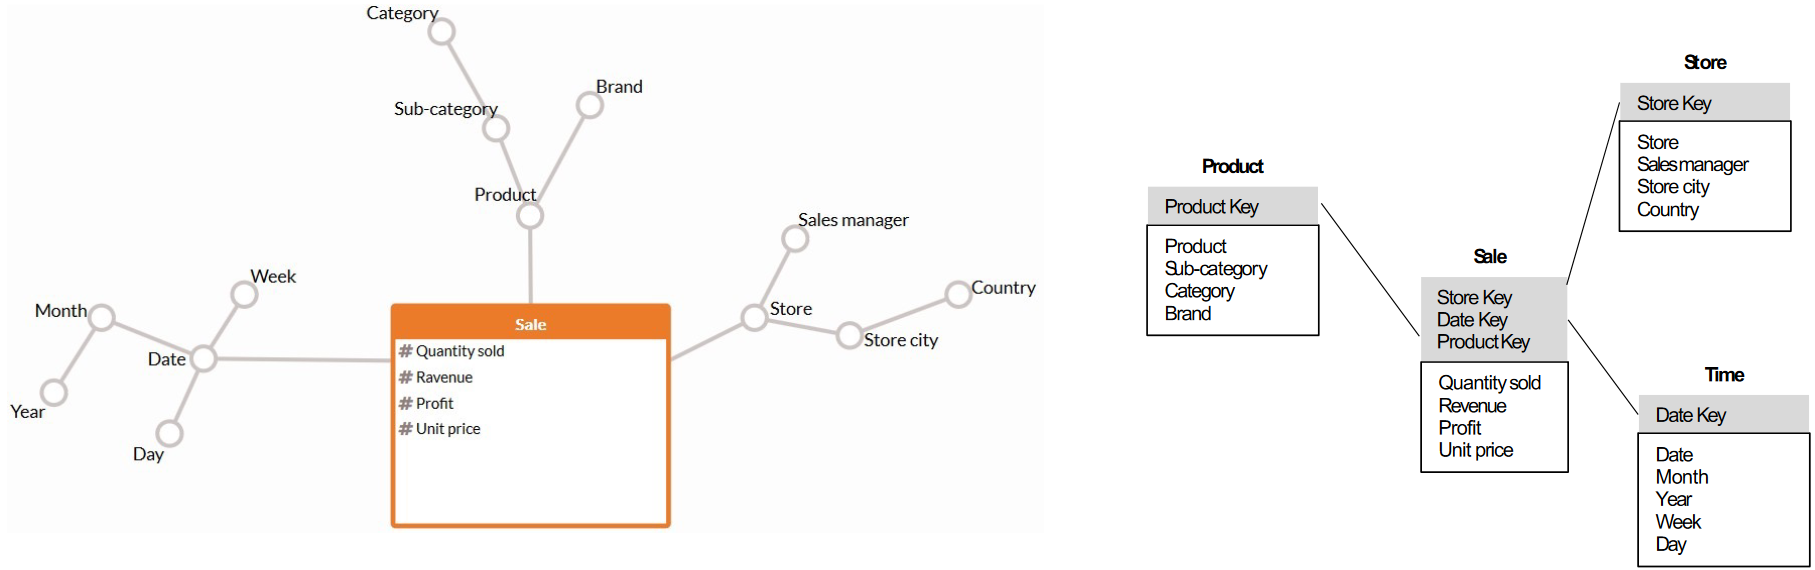
\includegraphics[width=\textwidth]{img/logical_star_schema.png}
            \caption{Example of star schema}
        \end{figure}

    \item[Snowflake schema] \marginnote{Snowflake schema}
        A star schema variant with partially normalized dimensional tables.
        \begin{figure}[H]
            \centering
            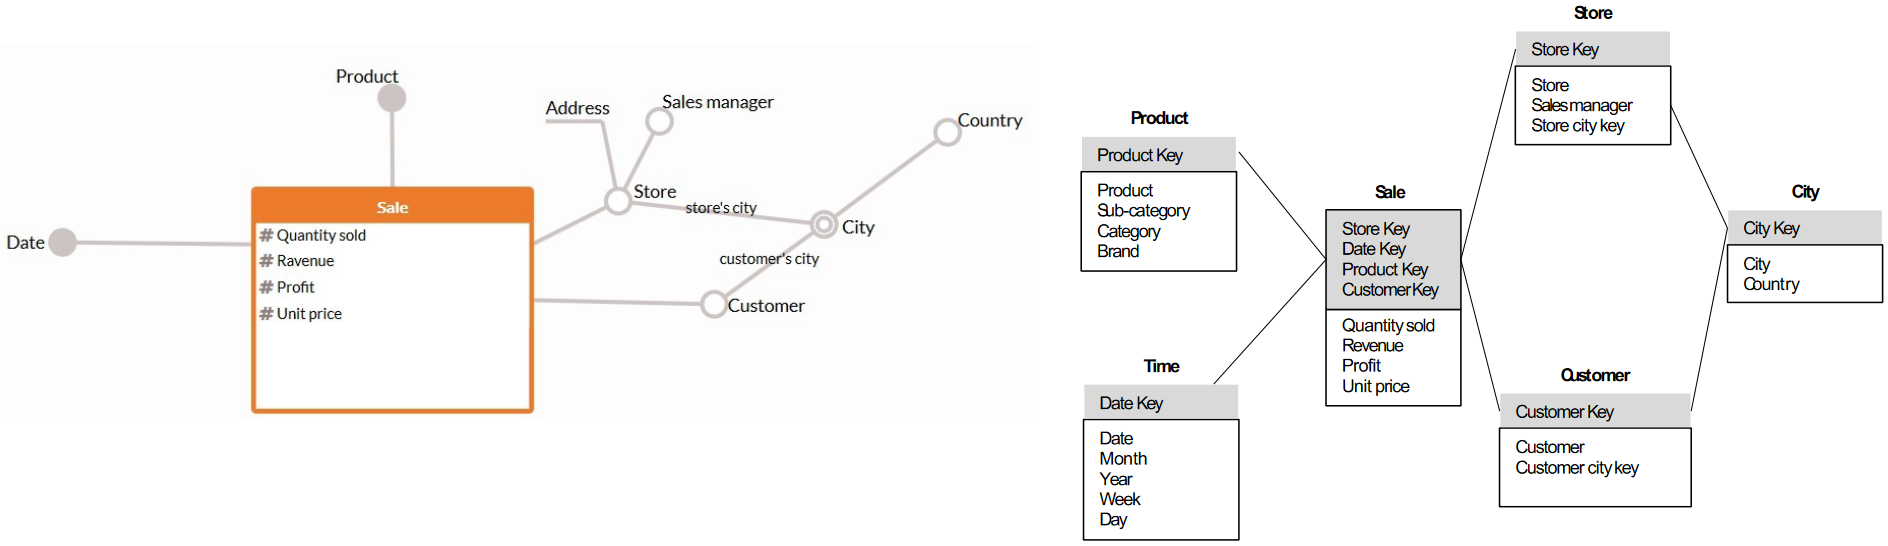
\includegraphics[width=\textwidth]{img/logical_snowflake_schema.png}
            \caption{Example of snowflake schema}
        \end{figure}
\end{descriptionlist}
    \chapter{Data lake}

\begin{description}
    \item[Dark data] \marginnote{Dark data}
        Acquired and stored data that are never used for decision-making processes.

    \item[Data lake] \marginnote{Data lake}
        Repository to store raw (unstructured) data.
        It has the following features:
        \begin{itemize}
            \item Does not enforce a schema on write.
            \item Allows flexible access and applies schemas on read.
            \item Single source of truth.
            \item Low cost and scalable.
        \end{itemize}

    \item[Storage]
        Stored data can be classified as:
        \begin{descriptionlist}
            \item[Hot] \marginnote{Hot storage}
                A low volume of highly requested data that require low latency.
                More expensive HW/SW.
            \item[Cold] \marginnote{Cold storage}
                A large amount of data that does not have latency requirements.
                Less expensive.
        \end{descriptionlist}

        \begin{figure}[ht]
            \centering
            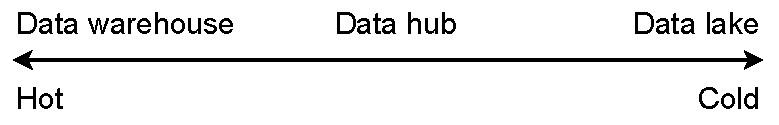
\includegraphics[width=0.5\textwidth]{img/_storage.pdf}
            \caption{Data storage technologies}
        \end{figure}
\end{description}


\section{Traditional vs insight-driven data systems}
\begin{tabular}{c | p{0.4\textwidth} | p{0.4\textwidth}}
    & \textbf{\makecell[c]{Traditional (data warehouse)}} & \textbf{\makecell[c]{Insight-driven (data lake)}} \\
    \hline
    \textbf{Sources} & Structured data & Structured, semi-structured and unstructured data \\
    \hline
    \textbf{Storage} & Limited ingestion and storage capability & Virtually unlimited ingestion and storage capability \\
    \hline
    \textbf{Schema} & Schema designed upfront & Schema not fixed \\
    \hline
    \textbf{Transformations} & \ac{etl} upfront & Transformations on query \\
    \hline
    \textbf{Analytics} & SQL, \ac{bi} tools, full-text search & Traditional methods, self-service \ac{bi}, big data, machine learning, \dots \\
    \hline
    \textbf{Price} & High storage cost & Low storage cost \\
    \textbf{Performance} & Fast queries & Scalability/speed/cost tradeoffs \\
    \hline
    \textbf{Quality} & High data quality & Depends on the use case \\
\end{tabular}


\section{Data architecture evolution}
\begin{description}
    \item[Traditional data warehouse] \marginnote{Traditional data warehouse} 
        (i.e. in-house data warehouse)
        \begin{itemize}
            \item Structured data with predefined schemas.
            \item High setup and maintenance cost. Not scalable.
            \item Relational high-quality data.
            \item Slow data ingestion.
        \end{itemize}

    \item[Modern cloud data warehouse] \marginnote{Modern cloud data warehouse} 
        \phantom{}
        \begin{itemize}
            \item Structured and semi-structured data.
            \item Low setup and maintenance cost. Scalable and easier disaster recovery.
            \item Relational high-quality data and mixed data.
            \item Fast data ingestion if supported.
        \end{itemize}

    \item[On-premise big data] \marginnote{On-premise big data} 
        (i.e. in-house data lake)
        \begin{itemize}
            \item Any type of data with schemas on read.
            \item High setup and maintenance cost.
            \item Fast data ingestion.
        \end{itemize}

    \item[Cloud data lake] \marginnote{Cloud data lake} 
        \phantom{}
        \begin{itemize}
            \item Any type of data with schemas on read.
            \item Low setup and maintenance cost. Scalable and easier disaster recovery.
            \item Fast data ingestion.
        \end{itemize}
\end{description}


\section{Components}

\subsection{Data ingestion} 
\marginnote{Data ingestion}
    \begin{descriptionlist}
        \item[Workload migration]
            Inserting all the data from an existing source.
        \item[Incremental ingestion]
            Inserting changes since the last ingestion.
        \item[Streaming ingestion]   
            Continuously inserting data.
    \end{descriptionlist}

    \begin{description}
        \item[\Acl{cdc} (\Acs{cdc})] \marginnote{\Acl{cdc} (\Acs{cdc})}
            Mechanism to detect changes and insert the new data into the data lake (possibly in real-time).
    \end{description}

\subsection{Storage}
\begin{descriptionlist}
    \item[Raw] \marginnote{Raw storage}
        Immutable data useful for disaster recovery.
    \item[Optimized] \marginnote{Optimized storage}
        Optimized raw data for faster query.
    \item[Analytics] \marginnote{Analytics storage}
        Ready to use data.
\end{descriptionlist}

\begin{description}
    \item[Columnar storage] \phantom{}
        \begin{itemize}
            \item Homogenous data are stores contiguously.
            \item Speeds up methods that process entire columns (i.e. all the values of a feature).
            \item Insertion becomes slower.
        \end{itemize}

    \item[Data catalog]
        Methods to add descriptive metadata to a data lake.
        This is useful to prevent an unorganized data lake (data swamp).
\end{description}
        
\subsection{Processing and analytics} 
\marginnote{Processing and analytics}
\begin{descriptionlist}
    \item[Interactive analytics]
        Interactive queries to large volumes of data.
        The results are stored back in the data lake.
    \item[Big data analytics]
        Data aggregations and transformations.
    \item[Real-time analytics]   
        Streaming analysis.
\end{descriptionlist}


\section{Architectures}

\subsection{Lambda lake} 
\marginnote{Lambda lake}
\begin{description}
    \item[Batch layer] Receives and stores the data. Prepares the batch views for the serving layer.
    \item[Serving layer] Indexes batch views for faster queries.
    \item[Speed layer] Receives the data and prepares real-time views. The views are also stored in the serving layer.
\end{description}
\begin{figure}[ht]
    \centering
    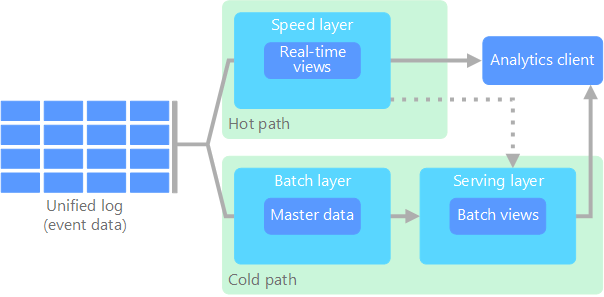
\includegraphics[width=0.5\textwidth]{img/lambda_lake.png}
    \caption{Lambda lake architecture}
\end{figure}

\subsection{Kappa lake} 
\marginnote{Kappa lake}
The data are stored in a long-term store.
Computations only happen in the speed layer (avoids lambda lake redundancy between batch layer and speed layer).
\begin{figure}[ht]
    \centering
    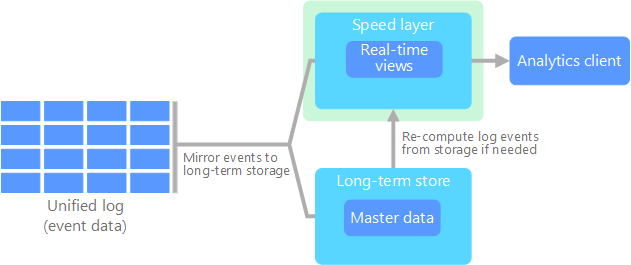
\includegraphics[width=0.5\textwidth]{img/kappa_lake.png}
    \caption{Kappa lake architecture}
\end{figure}

\subsection{Delta lake} 
\marginnote{Delta lake}
Framework that adds features on top of an existing data lake.
\begin{itemize}
    \item ACID transactions
    \item Scalable metadata handling
    \item Data versioning
    \item Unified batch and streaming
    \item Schema enforcement
\end{itemize}
\begin{figure}[ht]
    \centering
    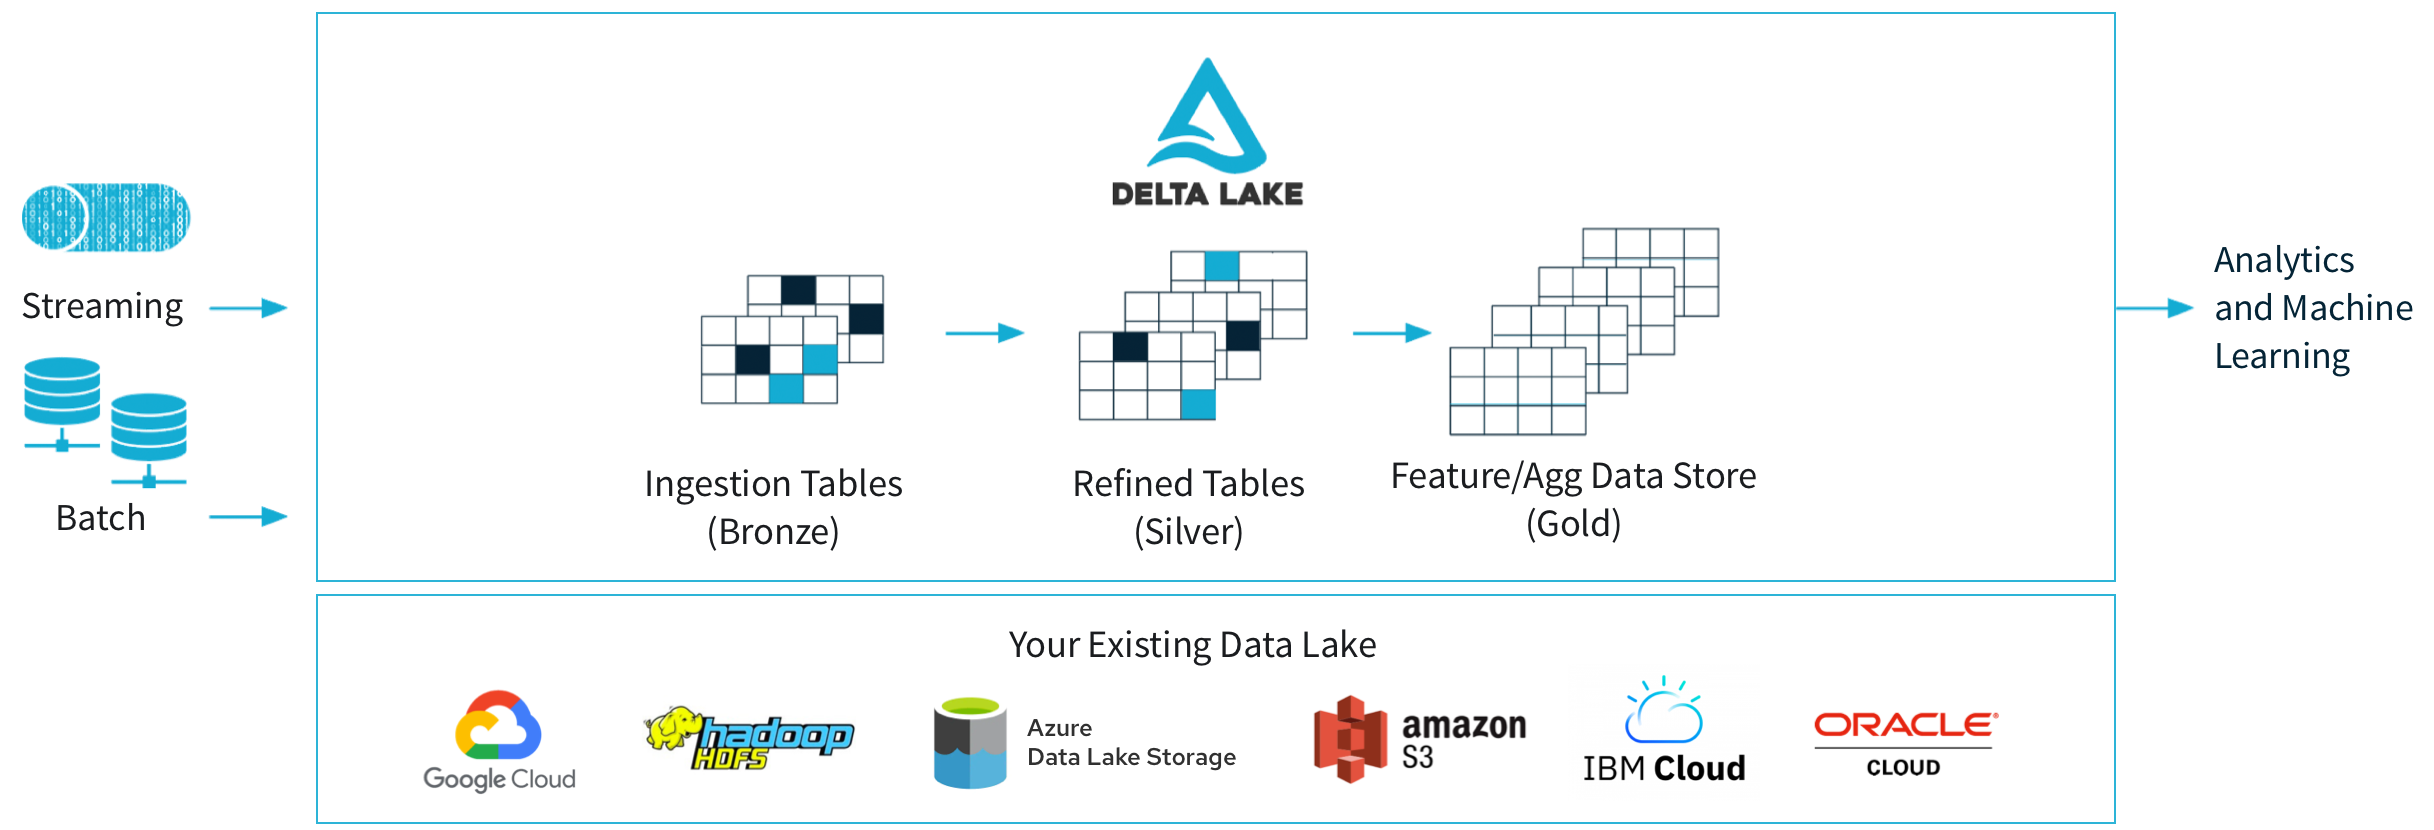
\includegraphics[width=0.7\textwidth]{img/delta_lake.png}
    \caption{Delta lake architecture}
\end{figure}


\section{Metadata}
\marginnote{Metadata}
Metadata are used to organize a data lake.
Useful metadata are:
\begin{descriptionlist}
    \item[Source] Origin of the data.
    \item[Schema] Structure of the data.
    \item[Format] File format or encoding.
    \item[Quality metrics] (e.g. percentage of missing values).
    \item[Lifecycle] Retention policies and archiving rules.
    \item[Ownership] 
    \item[Lineage] History of applied transformations or dependencies.
    \item[Access control] 
    \item[Classification] Sensitivity level of the data.
    \item[Usage information] Record of who accessed the data and how it is used.
\end{descriptionlist}
    \chapter{CRISP-DM}

\begin{description}
    \item[\Acl{crisp}] \marginnote{\acs{crisp}}
        Standardized process for data mining.
        \begin{figure}[ht]
            \centering
            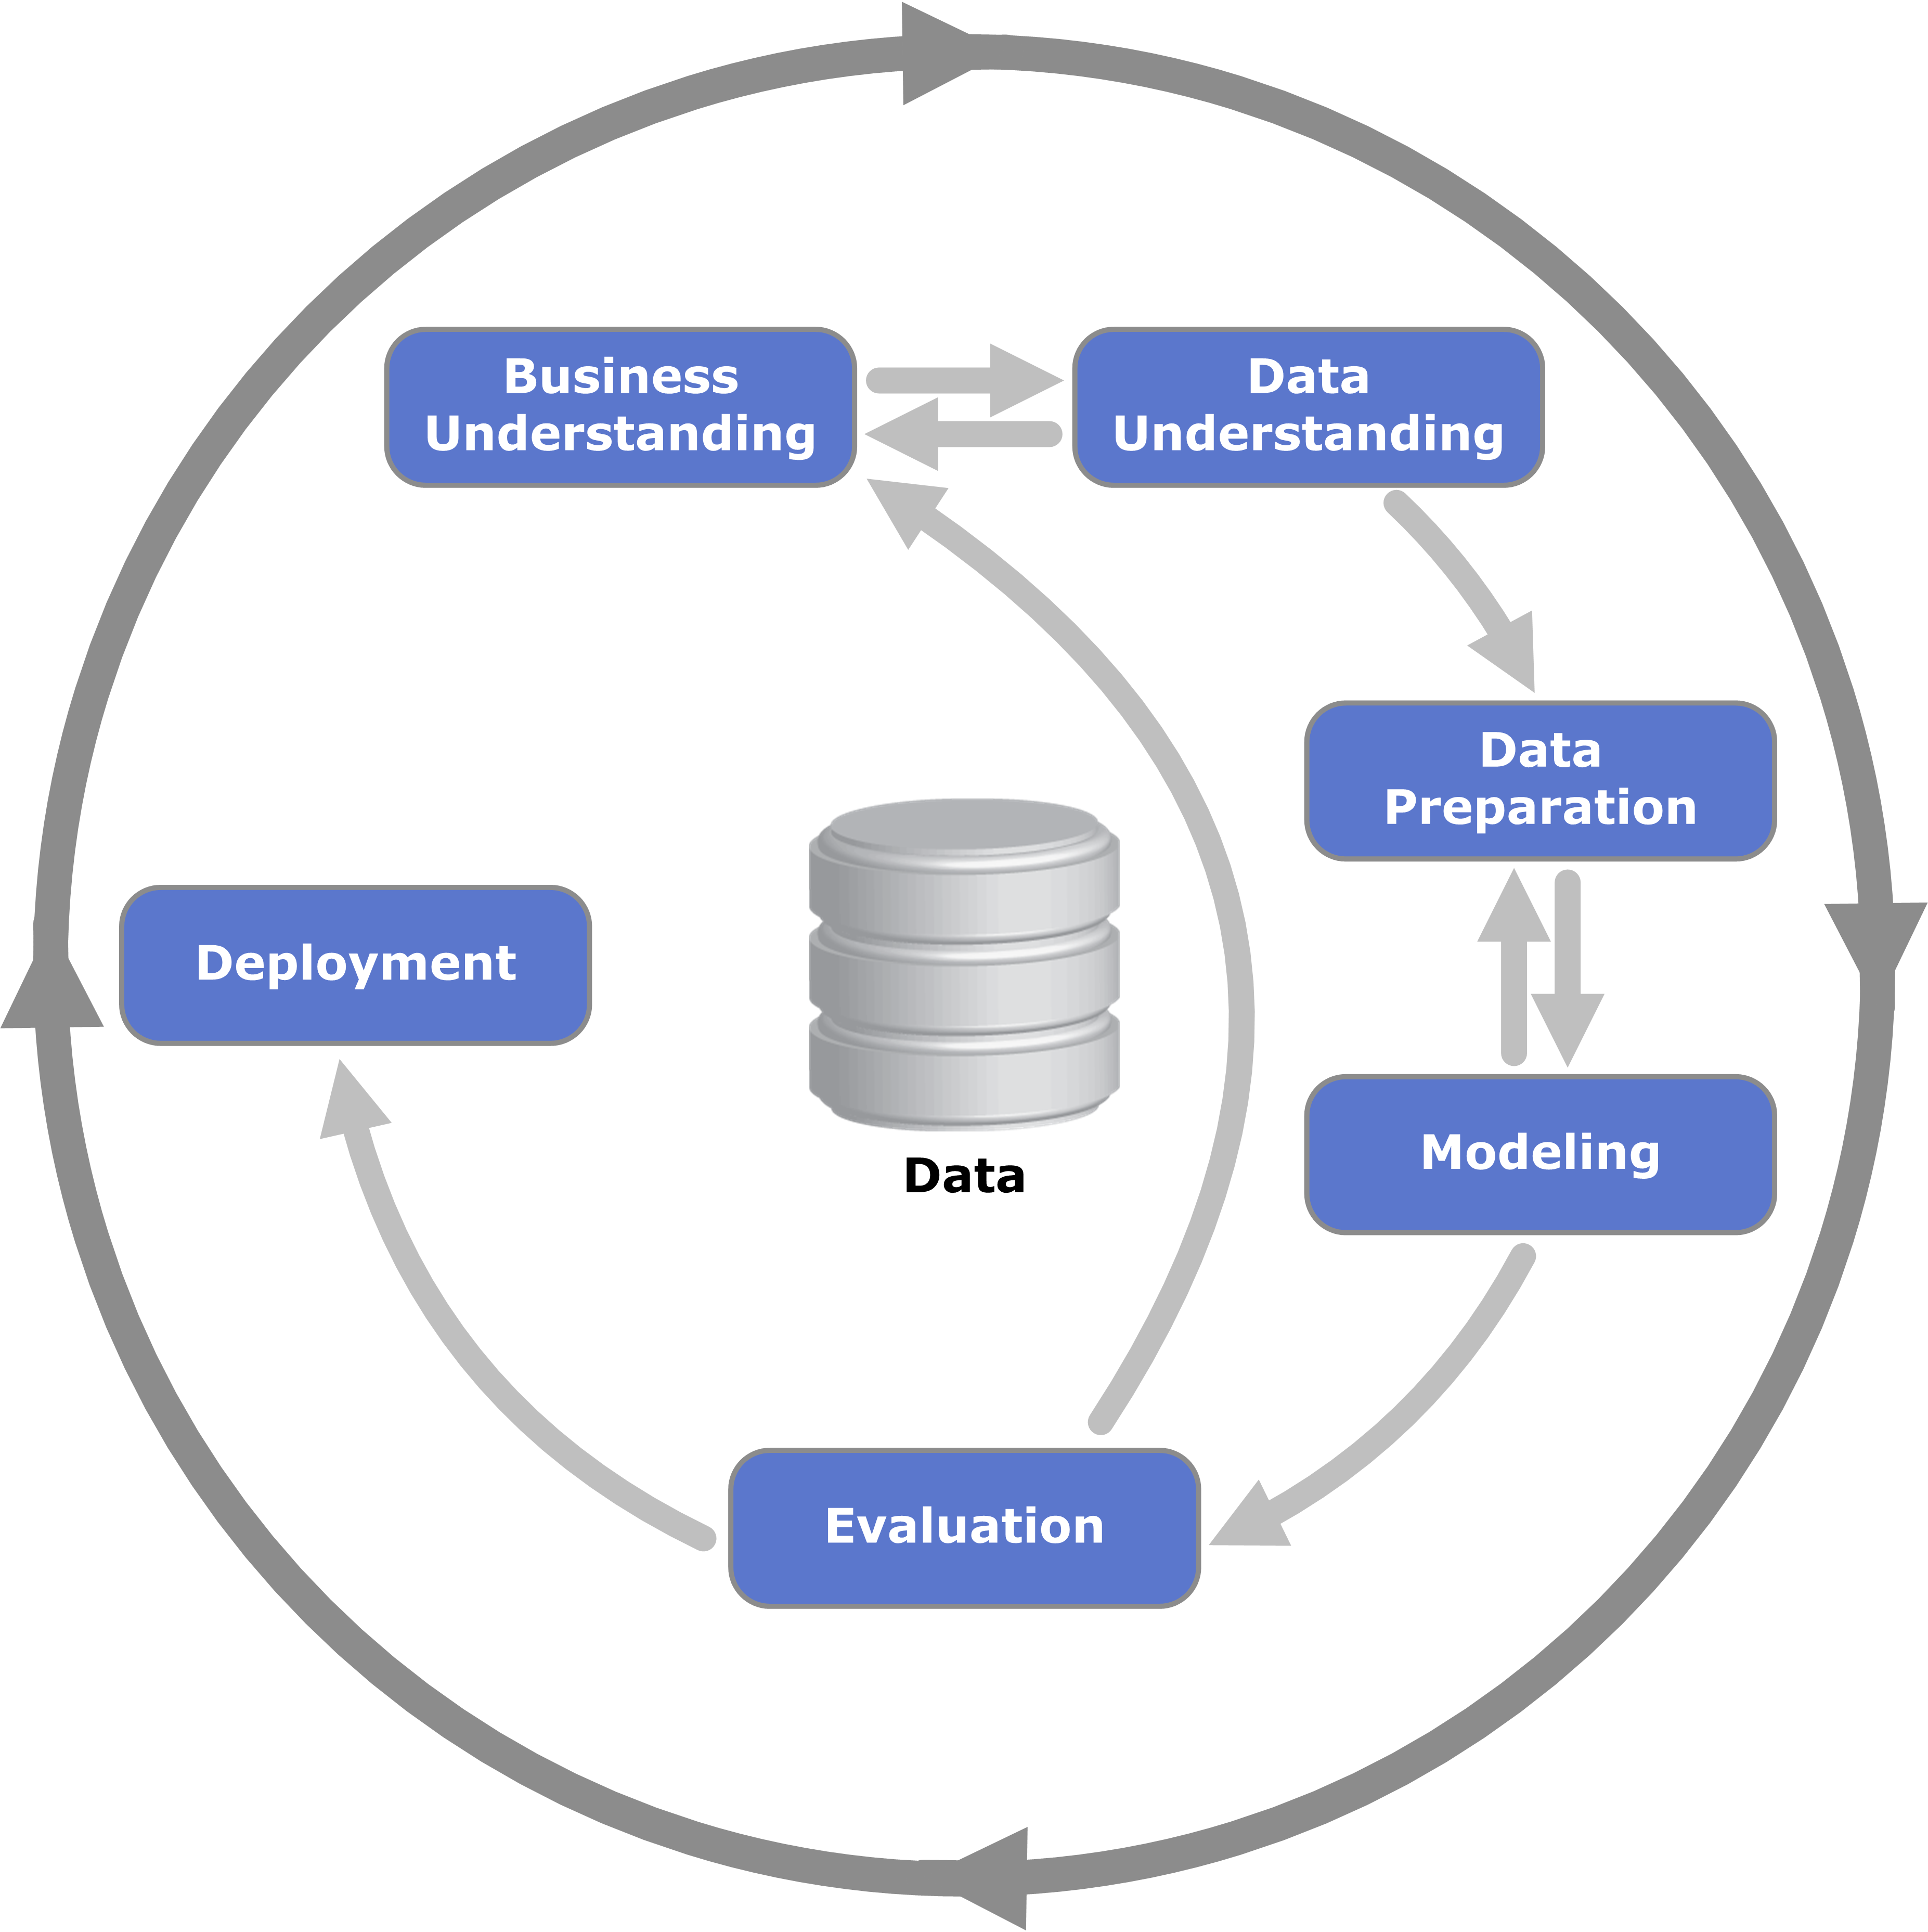
\includegraphics[width=0.45\textwidth]{img/crisp.png}
            \caption{\ac{crisp} workflow}
        \end{figure}
\end{description}


\section{Business understanding}
\begin{itemize}
    \item Determine the objective and the success criteria.
    \marginnote{Business understanding}
    \item Feasibility study.
    \item Produce a plan.
\end{itemize}

\section{Data understanding}
\begin{itemize}
    \item Determine the available (raw) data.
    \marginnote{Data understanding}
    \item Determine the cost of the data.
    \item Collect, describe, explore and verify data.
\end{itemize}

\section{Data preparation}
\begin{itemize}
    \item Data cleaning.
    \marginnote{Data preparation}
    \item Data transformations.
\end{itemize}

\section{Modeling}
\begin{itemize}
    \item Select modeling technique.
    \marginnote{Modeling}
    \item Build/train the model.
\end{itemize}

\section{Evaluation}
\begin{itemize}
    \item Evaluate results.
    \marginnote{Evaluation}
    \item Review process.
\end{itemize}

\section{Deployment}
\begin{itemize}
    \item Plan deployment.
    \marginnote{Deployment}
    \item Plan monitoring and maintenance.
    \item Final report and review.
\end{itemize}

    \chapter{Machine learning}


\section{Models}

\begin{description}
    \item[Function model] \marginnote{Function model}
        The model (predictor) is a deterministic function:
        \[ f: \mathbb{R}^D \rightarrow \mathbb{R} \]

        In this course, only linear functions are considered:
        \[ f_\vec{\uptheta}(\vec{x}) = \uptheta_0 + \uptheta_1 x_1 + \dots + \uptheta_D x_D = \vec{\uptheta}^T \vec{x} \]
        where $\vec{x} = \begin{pmatrix} 1, x_1, \dots, x_D \end{pmatrix}$ is the input vector and
        $\vec{\uptheta} = \begin{pmatrix} \uptheta_0, \dots, \uptheta_D \end{pmatrix}$ is the parameter vector.

    \item[Probabilistic model] \marginnote{Probabilistic model}
        The model is a multivariate probabilistic distribution.
\end{description}



\section{Learning}

\subsection{Empirical risk minimization}
\marginnote{Empirical risk minimization}
Used for function models.

Let $(\vec{x}_n, y_n)$ be a dataset of $N$ elements
where $\vec{x}_n \in \mathbb{R}^D$ are the examples and $y_n \in \mathbb{R}$ are the labels.
We want to estimate a predictor $f_\vec{\uptheta}(\vec{x}) = \vec{\uptheta}^T \vec{x}$ with parameters $\vec{\uptheta}$
such that, with the ideal parameters $\vec{\uptheta}^*$, it fits the data well:
\[ f_{\vec{\uptheta}^*}(\vec{x}_n) \approx y_n \]

We denote the output of the estimator as $\hat{y}_n = f_\vec{\uptheta}(\vec{x}_n)$.

\begin{description}
    \item[Loss function] \marginnote{Loss function}
        A loss function $\ell(y_n, \hat{y}_n)$ indicates how a predictor fits the data.

        An assumption commonly made in machine learning is that 
        the dataset $(\vec{x}_n, y_n)$ is independent and identically distributed. 
        Therefore, the empirical mean is a good estimate of the population mean.

        \begin{description}
            \item[Empirical risk] \marginnote{Empirical risk}
                Given the example matrix $\matr{X} = \begin{pmatrix} \vec{x}_1, \dots, \vec{x}_N \end{pmatrix} \in \mathbb{R}^{N \times D}$
                and the label vector $\vec{y} = \begin{pmatrix} y_1, \dots, y_N \end{pmatrix} \in \mathbb{R}^N$.
                The empirical risk is given by the average loss:
                \[ \textbf{R}_\text{emp}(f_\vec{\uptheta}, \matr{X}, \vec{y}) = \frac{1}{N} \sum_{n=1}^{N} \ell(y_n, \hat{y}_n) \]

            \begin{example}[Least-squares loss] \marginnote{Least-squares loss}
                The least-squares loss is defined as:
                \[ \ell(y_n, \hat{y}_n) = (y_n - \hat{y}_n)^2 \]

                Therefore, the minimization task is:
                \[ 
                    \min_{\vec{\uptheta} \in \mathbb{R}^D} \frac{1}{N} \sum_{n=1}^{N} (y_n - f_\vec{\uptheta}(\vec{x}_n))^2 =
                    \min_{\vec{\uptheta} \in \mathbb{R}^D} \frac{1}{N} \sum_{n=1}^{N} (y_n - \vec{\uptheta}^T\vec{x}_n)^2 =
                    \min_{\vec{\uptheta} \in \mathbb{R}^D} \frac{1}{N} \Vert \vec{y} - \matr{X}\vec{\uptheta} \Vert^2
                \]
            \end{example}

            \item[Expected risk] \marginnote{Expected risk}
                The expected risk is defined as:
                \[ \textbf{R}_\text{true}(f_\vec{\uptheta}) = \mathbb{E}_{\vec{x}, y}[\ell(y, f_\vec{\uptheta}(\vec{x}_\text{test}))] \]
                where the parameters $\vec{\uptheta}$ are fixed and the samples are taken from a test set.

            \item[Overfitting] \marginnote{Overfitting}
                A predictor $f_\vec{\uptheta}$ is overfitting when $\textbf{R}_\text{emp}(f, \matr{X}_\text{train}, \vec{y}_\text{train})$
                underestimates $\textbf{R}_\text{true}(f_\vec{\uptheta})$ (i.e. the loss on the training set is low, but on the test set is high).

            \item[Regularization] \marginnote{Regularization}
                Method that introduces a penalty term to the loss that
                helps to find a compromise between the accuracy and the complexity of the solution:
                \[ \bar{\ell}(y_n, \hat{y}_n) = \ell(y_n, \hat{y}_n) + \lambda \mathcal{R}(\vec{\uptheta}) \]
                where $\lambda \in \mathbb{R}^+$ is the regularization parameter and $\mathcal{R}$ is the penalty.
        \end{description}
\end{description}



\subsection{Maximum likelihood}
\marginnote{Maximum likelihood}
Used for probabilistic models.

\end{document}